\documentclass[aspectratio=169,t,11pt,table]{beamer}
\usepackage{../../slides,../../math}
\definecolor{accent}{HTML}{2B5269}
\definecolor{accent2}{HTML}{9D2235}

\title{Extra Slides for Topic 3: Selection on Observables}
\subtitle{\it  ECON 5783 — University of Arkansas}
\date{Fall 2024}
\author{Prof. Kyle Butts}
\begin{document}

\subsection{What controls to include?}

\begin{frame}{Good and bad controls}
  Which of these variables would you control for? Think identification and efficiency

  \bigskip
  \begin{columns}[t]
    \begin{column}{0.25\textwidth}
      \centering
      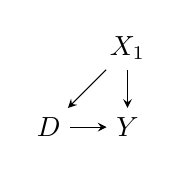
\begin{tikzpicture}[>=stealth, node distance=2cm]
        \node (X1) at (1,1) {$X_1$};
        \node (D) at (0,0) {$D$};
        \node (Y) at (1,0) {$Y$};
        
        \draw[->] (X1) -- (D);
        \draw[->] (X1) -- (Y);
        \draw[->] (D) -- (Y);
      \end{tikzpicture}

      \onslide<2>{\small $X_1$ Necessary for identification}
    \end{column}

    \begin{column}{0.25\textwidth}
      \centering
      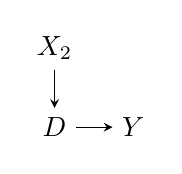
\begin{tikzpicture}[>=stealth, node distance=2cm]
        \node (X2) at (0,1) {$X_2$};
        \node (D) at (0,0) {$D$};
        \node (Y) at (1,0) {$Y$};
        
        \draw[->] (X2) -- (D);
        \draw[->] (D) -- (Y);
      \end{tikzpicture}

      \onslide<2>{\small $X_2$ Bad for efficiency (but may be good for robustness)}
    \end{column}

    \begin{column}{0.25\textwidth}
      \centering
      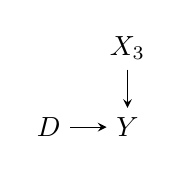
\begin{tikzpicture}[>=stealth, node distance=2cm]
        \node (X3) at (1,1) {$X_3$};
        \node (D) at (0,0) {$D$};
        \node (Y) at (1,0) {$Y$};
        
        \draw[->] (X3) -- (Y);
        \draw[->] (D) -- (Y);
      \end{tikzpicture}

      \onslide<2>{\small $X_3$ Good for efficiency}
    \end{column}

    \begin{column}{0.25\textwidth}
      \centering
      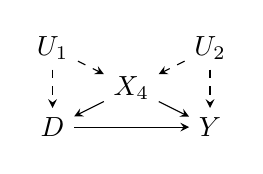
\begin{tikzpicture}[>=stealth, node distance=2cm]
        \node (U1) at (0,1) {$U_1$};
        \node (U2) at (2,1) {$U_2$};
        \node (X4) at (1,0.5) {$X_4$};
        \node (D) at (0,0) {$D$};
        \node (Y) at (2,0) {$Y$};
        
        \draw[->] (X4) -- (D);
        \draw[->] (X4) -- (Y);
        \draw[->] (D) -- (Y);
        
        \draw[->, dashed] (U1) -- (D);
        \draw[->, dashed] (U1) -- (X4);
        \draw[->, dashed] (U2) -- (X4);
        \draw[->, dashed] (U2) -- (Y);  
      \end{tikzpicture}

      \onslide<2>{\small $X_4$ ``Collider,'' generates bias (but may serve as proxy for $U_2$ if $U_2$ affects $D$)}
    \end{column}
  \end{columns}
\end{frame}

\begin{frame}{Good and bad controls}
  Which of these variables would you control for? Think identification and efficiency

  \bigskip
  \begin{columns}[t]
    \begin{column}{0.33\textwidth}
      \centering
      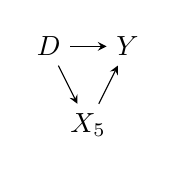
\begin{tikzpicture}[>=stealth, node distance=2cm]
        \node (D) at (0,1) {$D$};
        \node (Y) at (1,1) {$Y$};
        \node (X5) at (0.5,0) {$X_5$};
        
        \draw[->] (D) -- (Y);
        \draw[->] (D) -- (X5);
        \draw[->] (X5) -- (Y);
      \end{tikzpicture}
      
      \onslide<2>{\small $X_5$ Bad control, generate bias}
    \end{column}

    \begin{column}{0.33\textwidth}
      \centering
      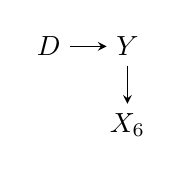
\begin{tikzpicture}[>=stealth, node distance=2cm]
        \node (D) at (0,1) {$D$};
        \node (Y) at (1,1) {$Y$};
        \node (X6) at (1,0) {$X_6$};
        
        \draw[->] (D) -- (Y);
        \draw[->] (Y) -- (X6);
      \end{tikzpicture}
      
      \onslide<2>{\small $X_6$ Bad control, generate bias}
    \end{column}

    \begin{column}{0.33\textwidth}
      \centering
      \begin{tikzpicture}[>=stealth, node distance=2cm]
        \node (D) at (0,1) {$D$};
        \node (Y) at (1,1) {$Y$};
        \node (X7) at (0,0) {$X_7$};
        
        \draw[->] (D) -- (Y);
        \draw[->] (D) -- (X7);
      \end{tikzpicture}

      \onslide<2>{\small $X_7$ Exercise for you}
    \end{column}
  \end{columns}
\end{frame}

\subsection{Proof of Unconfoundedness given propensity score}


\begin{frame}{Proof}
  This proof is from Imbens (2005, RESTAT) (may skip in class). 
  
  Show $\prob{D_i = 1}{Y_i(0), Y_i(1), \pi(\bm{X}_i)} = \prob{D_i = 1}{\pi(\bm{X}_i)} = \pi(\bm{X})_i$ which implies that $D_i$ and the potential outcomes are independent conditional on the propensity score
\end{frame}

\begin{frame}{Proof}
  \vspace*{-2\bigskipamount}
  \begin{align*}
    \prob{D_i = 1}{Y_i(0), Y_i(1), \pi(\bm{X}_i)} 
    &= \expec{D_i = 1}{Y_i(0), Y_i(1), \pi(\bm{X}_i)} \\ 
    &= \expec{\expec{D_i = 1}{Y_i(0), Y_i(1), \pi(\bm{X}_i), \bm{X}_i}}{Y_i(0), Y_i(1), \pi(\bm{X}_i)} \\
    &= \expec{\expec{D_i = 1}{Y_i(0), Y_i(1), \bm{X}_i}}{Y_i(0), Y_i(1), \pi(\bm{X}_i)} \\
    &= \expec{\expec{D_i = 1}{\bm{X}_i}}{Y_i(0), Y_i(1), \pi(\bm{X}_i)} \\
    &= \expec{\pi(\bm{X}_i)}{Y_i(0), Y_i(1), \pi(\bm{X}_i)} = \pi(\bm{X}_i),
  \end{align*}
  where 1st equality comes from $D_i$ being a 0/1 variable, 2nd from LIE, 4th from CIA (conditional on $\bm{X}$), and fifth from definition of the propensity score
\end{frame}


\subsection{Why not simple linear covariate adjustment?}

\begin{frame}{Simplest regression}
  Say the data-generating model is given by
  $$
    y_i = D_i \tau_i + W_i' \beta + u_i
  $$
  \begin{itemize}
    \item Effects of treatment, $\tau_i$, can vary arbitrarily by individuals

    \item $D_i$ is a treatment variable and $W_i$ is a vector of controls
  \end{itemize}
\end{frame}

\end{document}
